\cotefile{147}

\scanpage{54}
\mspage{26}
b) $h_1=1$, donc $\dim\operatorname{mod}G=\nu$, on veut $0\leq\nu\leq2$. On voit que le graphe $G$ a au maximum un bout, tous les autres sommets étant donc d'ordre $3$. \deleted{\unsure{Et}} Mais un graphe \inserted{\unsure{(top compact)|(top. compact)}} avec $h_1=1$ et n'ayant qu'un seul bout top. est homéom. \unsure{à|:}
\figure{\begin{tikzpicture}[x=1cm,y=1cm,baseline=-.1cm]
\draw (0,0) .. controls (-1.5,-.8) and (-1.3,1) .. (-.45,.7) .. controls (-.1,.65) and (0,.3) .. (0,0);\draw (0,0)--(1,0.04);\fill (0,0) circle (1.6pt);\fill (1,.04) circle (1.6pt);
\end{tikzpicture}},
et si \deleted{\unsure{il n'y a pas}} \inserted{$G$ n'a pas} de \unsure{sommets|sommet} d'ordre $2$, c'est qu'il est \inserted{isom\unsure{.}} au graphe \deleted{\unsure{qui}} combinatoire correspondant à la figure précédente. D'autre part, si le graphe n'a pas de bout, c'est qu'il est homéom. au cercle. Tous ses sommets sont d'ordre $2$, donc de poids marqué $1$, le nb de ces sommets \deleted{de} (il doit \unsure{en avoir} au moins $1$) est \inserted{donc} $1$ \unsure{ou} $2$, ce qui donne
\figure{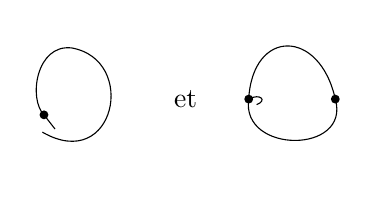
\begin{tikzpicture}[baseline=-.1cm]
\draw (-.02,-.22) .. controls (.9,-.75) and (1.2,.7) .. (.35,.85) .. controls (-.1,.9) and (-.2,.2) .. (0,0);\draw (0,0)--(.14,-.18);\fill (0,0) circle (1.6pt);
\node at (1.8,.2) {et};
\draw (2.6,.2) .. controls (2.65,1.1) and (3.5,1.1) .. (3.7,.2) .. controls (3.9,-.5) and (2.5,-.5) .. (2.6,.2);\draw (2.6,.2) .. controls (2.75,.28) and (2.84,.18) .. (2.70,.13);\fill (2.6,.2) circle (1.6pt);\fill (3.7,.2) circle (1.6pt);
\end{tikzpicture}}.
En résumé, on trouve encore trois cas :
\figure{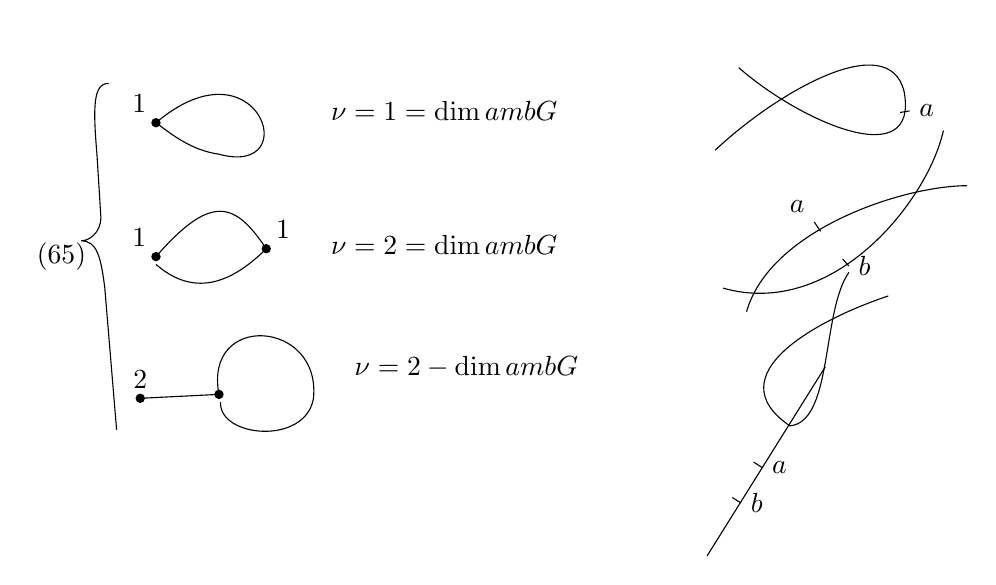
\begin{tikzpicture}[x=1cm,y=1cm]
\node at (-1.2,-1.7) {$(65)$};
\draw (-.6,.5) .. controls (-.8,.5) and (-.8,.2) .. (-.75,-.4) -- (-.7,-1.2) .. controls (-.7,-1.4) and (-.85,-1.5) .. (-.95,-1.5) .. controls (-.75,-1.5) and (-.7,-1.7) .. (-.65,-2.1) -- (-.5,-3.9);
\draw (0,0) .. controls (1.3,1.1) and (1.9,-.7) .. (.8,-.4) .. controls (.45,-.35) and (.2,-.15) .. (0,0);\fill (0,0) circle (1.7pt);\node[above left] at (0,0) {$1$};\node[right] at (2.1,.15) {$\nu=1=\dim\operatorname{amb}G$};
\draw (0,-1.7) .. controls (.7,-.9) and (1,-1) .. (1.4,-1.6) .. controls (.8,-2.2) and (.35,-2.1) .. (0,-1.80);\fill (0,-1.7) circle (1.7pt);\fill (1.4,-1.6) circle (1.7pt);\node[above left] at (0,-1.7) {$1$};\node[above right] at (1.4,-1.6) {$1$};\node[right] at (2.1,-1.55) {$\nu=2=\dim\operatorname{amb}G$};
\draw (-.2,-3.5)--(.8,-3.45);\draw (.8,-3.45) .. controls (.6,-2.4) and (2.1,-2.5) .. (2,-3.5) .. controls (1.9,-4.1) and (.8,-4) .. (.82,-3.55);\fill (-.2,-3.5) circle (1.7pt);\fill (.8,-3.45) circle (1.7pt);\node[above] at (-.2,-3.5) {$2$};\node[right] at (2.4,-3.1) {$\nu=2-\dim\operatorname{amb}G$};
\draw (7.4,.7) .. controls (8.2,0) and (9.7,-.65) .. (9.5,.4) .. controls (9.3,1.2) and (7.9,.4) .. (7.1,-.35);\draw (9.45,.13)--(9.57,.15);\node[right] at (9.57,.15) {$a$};
\draw (7.5,-2.4) .. controls (7.8,-1.35) and (9.5,-.8) .. (10.3,-.8);\draw (7.2,-2.1) .. controls (8.6,-2.5) and (9.8,-1) .. (10,-.1);\draw (8.44,-1.38)--(8.36,-1.26);\node[above left] at (8.36,-1.26) {$a$};\draw (8.72,-1.73)--(8.8,-1.82);\node[right] at (8.8,-1.82) {$b$};
\draw (7,-5.5)--(8.5,-3.1);\draw (8.05,-3.85) .. controls (7.1,-3.2) and (8.4,-2.5) .. (9.3,-2.2);\draw (8.05,-3.85) .. controls (8.6,-3.8) and (8.45,-2.4) .. (8.8,-1.9);\draw (7.7,-4.38)--(7.59,-4.31);\node[right] at (7.7,-4.38) {$a$};\draw (7.43,-4.83)--(7.32,-4.76);\node[right] at (7.43,-4.83) {$b$};
\end{tikzpicture}}
\margin{53}

\scanpage{56}
\mspage{27}
Revenons au cas d'un MD-graphe général, $\underline G$ sa dimension modulaire est
\[
\text{(67)}\qquad\delta(G)=\sum_{\alpha\in S}\underbrace{\bigl(3(g_\alpha-1)+\nu_\alpha+\widetilde\mu_\alpha\bigr)}_{\delta_\alpha}
\]
si on veut qu'elle soit égale à $1$ ou $2$, cela signifie que l'on est dans l'un des deux cas :
\[
\left\{\begin{array}{l}
1\text{ ou }2\text{ des }\delta_\alpha\text{ sont égaux à }1,\text{ les autres sont nuls}\\
1\text{ des }\delta_\alpha\text{ est égal à }2,\text{ les autres sont nuls}
\end{array}\right.
\]
Le cas $\delta(G)=1$ correspond au cas où \unsure{exactement} un des $\delta_\alpha$ est $=1$, les autres étant nuls.

II) $\underline G$ \uline{de dim modulaire} $1$

Cela signifie qu'il existe un sommet $\alpha_0$ (et un seul, \deleted{de} fait) de $\underline G$ qui \deleted{soit de genre} \inserted{satisfasse la} condition
\[
\begin{aligned}
\text{(68)}\quad &(\alpha_0\text{ de genre }1,\text{ et son poids total }\nu_{\alpha_0}+\widetilde\mu_{\alpha_0}\text{ est ég. à }\unsure{1}\\
&\qquad\text{i.e. }\alpha_0\text{ est d'ordre }1,\text{ ou \unsure{sommet|point} isolé de poids marqué }1)\\
&\uline{\text{ou}}\quad(\alpha_0\text{ de genre }0,\text{ et son poids total }\nu_{\alpha_0}+\widetilde\mu_{\alpha_0}=4,\\
&\qquad\text{i.e. }(\nu_{\alpha_0},\widetilde\mu_{\alpha_0})\in\{(4,0),(3,1),(2,2),(1,3),(0,4)\})
\end{aligned}
\]
avec en plus
\[
\begin{aligned}
\text{(69)}\quad&\text{les sommets }\alpha\ne\alpha_0\text{ sont de genre }0,\\
&\text{d'ordre }\widetilde\mu_\alpha\leq3,\text{ et pour un tel }\alpha\text{ le poids}\\
&\text{marqué }\nu_\alpha\text{ est égal à }3-\widetilde\mu_\alpha.
\end{aligned}
\]
\deleted{On voit que la MD-structure d'un tel graphe}
\margin{55}

\scanpage{57}
\deleted{est \unsure{déterminée|déterminé} par la structure de graphe avec un sommet \unsure{pondérés|pondéré} \unsure{par le}}

Les cas les plus simples sont les cas élémentaires (graphes \deleted{à \unsure{un pt iso}} \inserted{ponctuels})
\margin{MD-graphes élémentaires (sommet isolé \inserted{i.e. codim modulaire nulle}) de dim. modulaire $1$ \deleted{\illegible{1}} \deleted{\unsure{de dim|ambiante}\ $1$}}
\figure{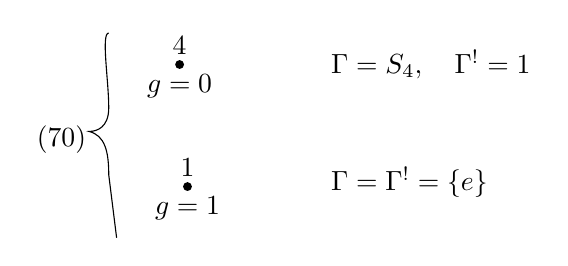
\begin{tikzpicture}[x=1cm,y=1cm]
\node at (-1.3,-.75) {$(70)$};\draw (-.7,.6) .. controls (-.8,.6) and (-.7,0) .. (-.7,-.35) .. controls (-.7,-.6) and (-.85,-.65) .. (-.95,-.65) .. controls (-.75,-.7) and (-.7,-.9) .. (-.7,-1.2) -- (-.6,-2);
\fill (.2,.2) circle(1.6pt);\node[above] at (.2,.2) {$4$};\node[below] at (.2,.2) {$g=0$};\node[right] at (2,.2) {$\Gamma=\mathfrak S_4,\quad\Gamma^!=1$};
\fill (.3,-1.35) circle(1.6pt);\node[above] at (.3,-1.35) {$1$};\node[below] at (.3,-1.35) {$g=1$};\node[right] at (2,-1.3) {$\Gamma=\Gamma^!=\{e\}$};
\end{tikzpicture}}
Les autres cas sont ceux des \inserted{MD-}graphes ``\uline{\unsure{rationnels|rétro-nuls}}'' (tous les $g_\alpha$ nuls) tels que tous les $\widehat\nu_\alpha$ soient égaux à trois (donc les sommets d'ordre $1\leq\widetilde\mu_\alpha\leq3$) \deleted{\unsure{et un}} \inserted{sauf l'}un d'eux, qui est égal à $4$ (donc $1\leq\widetilde\mu_{\alpha_0}\leq4$), ou bien des \inserted{MD-}graphes qui ont tous leurs sommets sauf un rationnels et $\widehat\nu_\alpha=3$, \deleted{(donc} sauf un \inserted{$\alpha_0$} qui est un sommet-bout ($\widetilde\mu_\alpha=1$) et de genre $1$, $\nu_{\alpha_0}=0$ --- donc ici tous les sommets sont d'ordre $1\leq\widetilde\mu_\alpha\leq3$, et les $\nu_\alpha$ \inserted{pour $\alpha\ne\alpha_0$} sont égaux à $3-\widetilde\mu_\alpha$, \deleted{pour $\alpha\ne$} et $\nu_{\alpha_0}=0$.

Dans l'un et l'autre cas \inserted{($g_{\alpha_0}=0$, $\unsure{g_{\alpha_0}|g_\alpha}=1$)} on aura un iso can. de multiplicités
\[
\text{(71)}\qquad\widehat M_G\simeq\widehat M_{g_{\alpha_0},\widehat I_{\alpha_0}}
\]
\margin{avec $\widehat I_{\alpha_0}=I_{\alpha_0}+\widetilde A_{\alpha_0}$ (de cardinal $4$ ou $1$, suivant que $g_{\alpha_0}=0$ ou $g_{\alpha_0}=1$)}
\margin{56}

\scanpage{58}
\mspage{28}
\deleted{\unsure{(72)|(71)}} et. l'action de $\Gamma_{\underline G}=\Gamma$ sur $\widehat M_G\simeq\widehat M_{g_{\alpha_0},\widehat I_{\alpha_0}}$ est triviale si $g_{\alpha_0}=1$, et elle se fait à travers
\diagram{\begin{tikzcd}[ampersand replacement=\&]
\text{(72)}\quad\Gamma_{\underline G}\arrow[r]\&\mathfrak S_{\widehat I_{\alpha_0}}\quad(\simeq\mathfrak S_4)
\end{tikzcd}}
dans le cas où $g_{\alpha_0}=0$. L'image de $\Gamma_{\underline G}$ dans $\mathfrak S_4$ doit pouvoir être n'importe quel sous-groupe de $\mathfrak S_4$, sauf erreur. Explicitons déjà quels sont les cas où la dim. ambiante est $\leq2$. Le cas de la dim ambiante $1$ \inserted{i.e. où la codim modulaire \inserted{$\unsure{s_1|\delta_1}$} de $\underline G$ est $0$,} est évidemment celui donné par (70), où $G$ est réduit à un sommet isolé.

Considérons donc le cas de la dim mod ambiante $2$, i.e. codim modulaire $1$, i.e. \uline{une} arête. On trouve soit
\figure{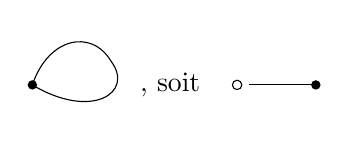
\begin{tikzpicture}[baseline=-.1cm]
\draw (0,0) .. controls (.2,.6) and (.75,.72) .. (1.0,.3) .. controls (1.3,-.1) and (.75,-.45) .. (0,0);
\fill (0,0) circle(1.7pt);\node at (1.75,0) {, soit};
\draw (2.75,0)--(3.6,0);\draw (2.6,0) circle(1.7pt);\fill (3.6,0) circle(1.7pt);
\end{tikzpicture}}.
\inserted{On trouve les trois cas de dim modulaire} \deleted{Dans le cas $g_{\alpha_0}=0$ tous les sommets sauf $1$ sont d'ordre} ambiante $2$, dim modulaire $1$
\margin{MD-graphes de dim mod $1$, dim. modulaire ambiante $2$.}
\figure{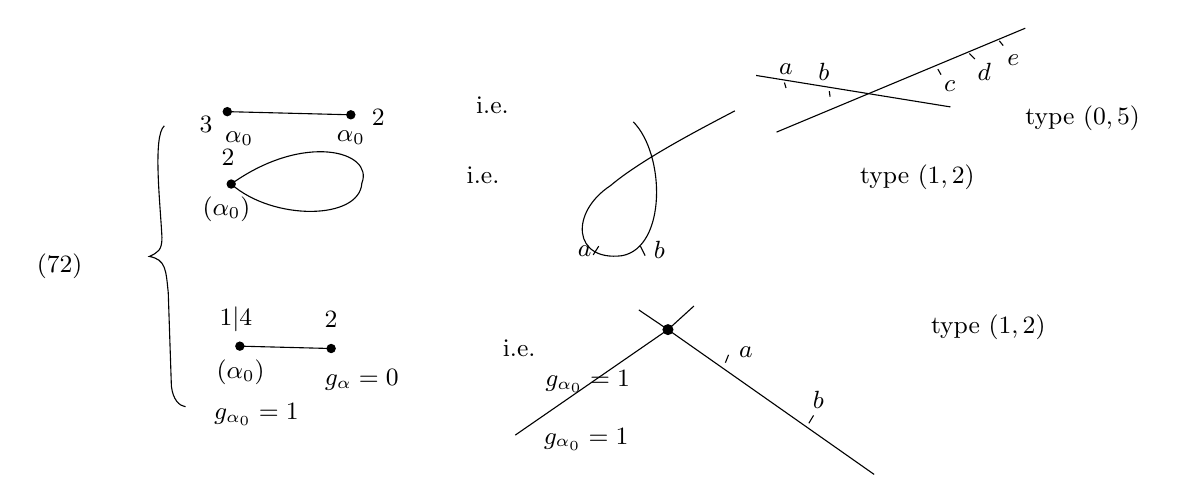
\begin{tikzpicture}[x=.010cm,y=-.010cm,every node/.style={font=\small}]
\node at (-150,310) {$(72)$};
\draw (-17,132) .. controls (-32,145) and (-22,232) .. (-20,274) .. controls (-20,290) and (-25,293) .. (-36,298) .. controls (-15,302) and (-15,315) .. (-12,344) -- (-8,463) .. controls (-6,480) and (2,488) .. (10,489);
% First graph and its curve.
\draw (63,114)--(220,118);\fill (63,114) circle(1.7pt);\fill (220,118) circle(1.7pt);
\node at (36,130) {$3$};\node at (78,148) {$\alpha_0$};\node at (255,122) {$2$};\node at (220,147) {$\deleted{\unsure{\alpha_0}}$};\node at (400,106) {i.e.};
\draw (735,68)--(982,108);\draw (761,140)--(1077,8);
\draw (771,77)--(773,84);\node at (773,60) {$a$};
\draw (828,88)--(829,95);\node at (821,64) {$b$};
\draw (966,60)--(970,67);\node at (981,82) {$c$};
\draw (1006,40)--(1013,47);\node at (1025,63) {$d$};
\draw (1044,24)--(1049,30);\node at (1062,48) {$e$};\node at (1150,123) {type $(0,5)$};
% Second graph and its curve.
\draw (68,206) .. controls (160,140) and (250,164) .. (234,205) .. controls (231,252) and (121,253) .. (68,206);\fill (68,206) circle(1.7pt);
\node at (64,172) {$2$};\node at (62,238) {$(\alpha_0)$};\node at (388,195) {i.e.};
\draw (579,127) .. controls (620,169) and (621,286) .. (565,297) .. controls (502,305) and (498,242) .. (550,208) .. controls (590,174) and (670,133) .. (708,113);
\draw (535,285)--(528,296);\node at (517,291) {$a$};\draw (588,285)--(594,297);\node at (612,290) {$b$};\node at (940,198) {type $(1,2)$};
% Third graph and its curve.
\draw (79,412)--(195,415);\fill (79,412) circle(1.7pt);\fill (195,415) circle(1.7pt);
\node at (74,378) {$\deleted{\unsure{1|4}}$};\node at (195,378) {$2$};\node at (80,445) {$(\alpha_0)$};\node at (100,499) {$g_{\alpha_0}=1$};\node at (234,455) {$g_\alpha=0$};\node at (434,414) {i.e.};
\draw (429,525)--(623,391)--(656,361);\draw (586,366)--(623,391)--(885,575);\fill (623,391) circle(2pt);
\node at (521,457) {$\deleted{\unsure{g_{\alpha_0}}=1}$};\node at (519,530) {$g_{\alpha_0}=1$};
\draw (696,433)--(700,423);\node at (722,420) {$a$};\draw (802,510)--(808,500);\node at (814,480) {$b$};\node at (1030,388) {type $(1,2)$};
\end{tikzpicture}}
(NB les sommets, ou branches des courbes, dont le genre \inserted{ou poids marqué} n'est pas marqué en dessous, sont de genre \inserted{ou poids marqué} zéro; les poids marqués sont indiqués sur le graphe \unsure{au|en} dessus des sommets)
\margin{57}

\scanpage{59}
Les groupes d'automorphismes de ces MD-graphes sont
\figure{\begin{tikzpicture}[x=1cm,y=1cm]
\node at (-1.25,-1) {$(73)$};\draw (-.7,.6) .. controls (-.9,.6) and (-.8,0) .. (-.8,-.5) .. controls (-.8,-.7) and (-.9,-.8) .. (-1,-.8) .. controls (-.8,-.9) and (-.8,-1.1) .. (-.75,-1.5) -- (-.65,-2.4);
\draw (0,.35)--(1.5,.35);\fill (0,.35) circle(1.5pt);\fill (1.5,.35) circle(1.5pt);\node[above] at (0,.35) {$3$};\node[above] at (1.5,.35) {$2$};\node[below] at (0,.35) {$\alpha_0$};\node[right] at (2.4,.4) {$\Gamma=\mathfrak S_3\times\mathfrak S_2,\quad\Gamma^!=1,\quad\operatorname{Im}(\Gamma\to\mathfrak S_4)\simeq\mathfrak S_3$};
\draw (0,-.85) .. controls (2,.3) and (2.25,-1.3) .. (1,-.95) -- (0,-.85);\fill (0,-.85) circle(1.5pt);\node[above] at (0,-.85) {$2$};\node[below] at (0,-.85) {$(\alpha_0)$};\node[right] at (2.4,-.8) {$\Gamma\simeq\mathfrak S_2\times\mathfrak S_2,\quad\Gamma^!\simeq\mathfrak S_2,\quad\operatorname{Im}(\Gamma\to\mathfrak S_4)\simeq\underset{\substack{\Vert\\\mathfrak S_2\times\mathfrak S_2}}\Gamma$};
\draw (0,-2.2)--(1.7,-2.2);\fill (0,-2.2) circle(1.5pt);\fill (1.7,-2.2) circle(1.5pt);\node[above] at (1.7,-2.2) {$2$};\node[below] at (0,-2.2) {$g_{\alpha_0}=1$};\node[right] at (2.4,-2.1) {$\Gamma\simeq\mathfrak S_2,\quad\Gamma^!\simeq1\quad\deleted{\unsure{\operatorname{Im}(\Gamma\to\mathfrak S_4)=1}}$};
\end{tikzpicture}}

$\overline{\underline{\mathrm{III}}}$) \uline{Dim. modulaire $2$}

Correspond par (67) aux deux cas suivants :

$1^\circ)$ Tous les $\alpha\in S$ sauf un seul \inserted{$\alpha_0$} sont de genre $0$, et de poids total $3$ (i.e. d'ordre \inserted{$\widetilde\mu_\alpha$} $\leq3$, et de poids marqué $3-\widetilde\mu_\alpha$), et $(\alpha_0,\widehat\nu_{\alpha_0})$ est d'un des deux types $(0,5)$, $(1,2)$ \deleted{\unsure{ou|et} $\unsure{(2,0)}$}, i.e. $\alpha_0$ est de genre $0$, d'ordre \inserted{$\widetilde\mu_{\alpha_0}$} $\leq5$ et de poids marqué $5-\widetilde\mu_{\alpha_0}$, \uline{ou} $\alpha_0$ de genre $1$, d'ordre \deleted{$\unsure{\leq2}$} \inserted{$\deleted{\unsure{\leq}}\;\widetilde\mu_\alpha\in\{1,2\}$} et de poids marqué $2-\widetilde\mu_{\alpha_0}\in\{1,0\}$.
\margin{donc deux cas en réalité}

$2^\circ)$ Tous les $\alpha=S$ sauf deux \unsure{exactement} $\alpha_0$ et $\alpha_1$, sont de genre $0$, \inserted{et} de poids total $3$ (i.e. d'ordre $1\leq\widetilde\mu_\alpha\leq3$, et de poids \deleted{\unsure{total}} marqué égal \unsure{à|:} $3-\widetilde\mu_\alpha$), $\alpha_0$ et $\alpha_1$ sont chacun \deleted{soit} de type $(\alpha_i,\widehat\mu_i)$ égal soit \unsure{à|:} $(0,4)$, soit à $(1,1)$.
\margin{Cela fait donc trois cas, suivant que les deux types de dim mod $1$ qui interviennent sont tous deux $(0,4)$, ou l'un $(0,4)$, l'autre $(1,1)$, ou tous deux $(1,1)$.}

La \deleted{\unsure{schéma|variété}} \inserted{mult.} modulaire $\widehat M_G$ est alors isomorphe, suivant les cas, à l'une des suivantes :
\margin{58}

\scanpage{60}
\mspage{29}
\margin{\deleted{\illegible{1}}multiplicités modulaires \inserted{$\widehat M_G$} de dim $2$}
\[
(74)\quad\left\{\begin{array}{ll}
\widehat M^!_{0,5}&\Gamma\text{ opère via }\Gamma\longrightarrow\mathfrak S_{\widehat I_{\alpha_0}}\ (\simeq\mathfrak S_5)\\
\widehat M^!_{1,2}&\Gamma\text{ --- }\quad\Gamma\longrightarrow\mathfrak S_{\widehat I_{\alpha_0}}\simeq\mathbb Z/2\mathbb Z\\
\widehat M^!_{0,4}\times\widehat M^!_{0,4}&\Gamma\text{ --- }\quad\Gamma\longrightarrow\deleted{\unsure{\prod_{\alpha\in\{\alpha_0,}}}\mathfrak S_{\deleted{\unsure{\widehat I}}\bigl(\widehat I_{\alpha_0}\amalg\widehat I_{\alpha_1}}\simeq\mathfrak S_8\\
\widehat M^!_{0,4}\times\widehat M^!_{1,1}&\Gamma\text{ --- }\quad\Gamma\longrightarrow\mathfrak S^{\deleted{\unsure{4|*}}}_{\widehat I_{\alpha_0}}\simeq\mathfrak S_4\\
\widehat M^!_{1,1}\times\widehat M^!_{1,1}&\Gamma\text{ opère trivialement.}
\end{array}\right.
\]

\uline{NB} \deleted{\unsure{à}} Dans le cas $3^\circ$) de $\widehat M_{0,4}\times\widehat M_{0,4}$, $\Gamma$ \deleted{opère}\inserted{s'envoie} dans $\mathfrak S_8$ par l'intermédiaire de
\[
\begin{array}{rcl}
\Gamma&\longrightarrow&\mathbb Z/2\mathbin{\cdot}(\mathfrak S_4\times\mathfrak S_4)\\
&&\text{prod. }\frac12\text{ direct}
\end{array}
\]

On peut considérer que par rapport aux schémas modulaires \inserted{$\widehat M_G$} de dim $1$, \deleted{\unsure{qui sont|savoir}}\inserted{\unsure{ils|qui} sont \unsure{deux|donc} :}
\margin{(cas élémentaires!)}
\[
(75)\quad\left\{\begin{array}{ll}
\widehat M^!_{0,4}&\Gamma\text{ opère via }\Gamma\longrightarrow\mathfrak S_{I_{\alpha_0}}\simeq\mathfrak S_4\\
\widehat M^!_{1,1}&\Gamma\text{ opère trivialt},
\end{array}\right.
\]
les ``cas \unsure{''|``}nouveaux'' de (74) sont $\widehat M^!_{0,5}$ et $\widehat M^!_{1,2}$.

Cela fait en tous essentiellement quatre cas ``élémentaires'' à étudier à fond, pour le cas \unsure{des|de} dim. modulaires $\leq2$. J'ai l'impression qu'une compréhension plus ou moins complète de la structure des $\Pi_1$ \inserted{discrets (i.e. dans le contexte analytique)} impliqués dans ces cas, \unsure{donnerait|donnera} la clef pour une compréhension complète dans le cas général.
\margin{59}

\scanpage{61}
Partant des MD-graphes ``élémentaires'' correspondants, je voudrais expliciter dans les quatre cas la structure \inserted{de spécialisation entre} des strates des $\widehat M_{g,\nu}$ et $\widehat M^!_{g,\nu}$.

8) \uline{Structure de spécialisation des strates en dim modulaire $\leq2$.}

$1^\circ)$ \uline{Cas \unsure{de|des}} $\widehat M^!_{0,4}$ \uline{et} $\widehat M_{0,4}$

Commençons par $\widehat M^!_{0,4}$.
\figure{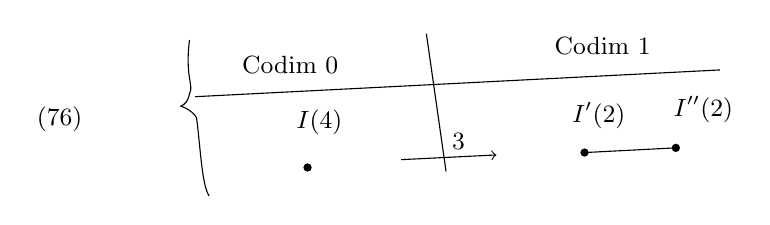
\begin{tikzpicture}[x=.010cm,y=-.010cm,every node/.style={font=\small}]
\node at (-183,33) {$(76)$};
\draw (-18,-68) .. controls (-24,-20) and (-12,-10) .. (-18,0) .. controls (-20,10) and (-23,13) .. (-29,16) .. controls (-17,20) and (-10,28) .. (-9,31) .. controls (-4,70) and (-2,118) .. (7,130);
\draw (-11,4)--(656,-30);\draw (283,-76)--(308,99);
\node at (110,-36) {Codim $0$};\node at (507,-61) {Codim $1$};
\node at (147,36) {$I(4)$};\fill (132,94) circle(1.5pt);
\draw[->] (251,84)--(372,78);\node at (324,61) {$3$};
\node at (502,28) {$I'(2)$};\node at (635,20) {$I''(2)$};
\draw (484,75)--(600,69);\fill (484,75) circle(1.5pt);\fill (600,69) circle(1.5pt);
\end{tikzpicture}}
Le diagramme signifie que l'ens. marqué $I$ de cardinal $4$, \inserted{\unsure{se partageant|se partage}} suivant l'une quelc. des trois partitions de $I$ en $I'$ et $I''$ de cardinal $2$ chacun, donne $3$ spécialisations différentes de la strate \unsure{maxima|maxim.} --- cela correspond bien sûr aux trois pts à l'infini de $U_{0,3}$

on aura
\[
(77)\qquad \widehat M^!_{0,4}\simeq\mathbb P^1_{\mathbb Z},\quad M^!_{0,4}\simeq(U_{0,3})_{\mathbb Z}=\mathbb P^1_{\mathbb Z}\smallsetminus\{0,1,\infty\}
\]
Pour bien faire, il faudrait aussi expliciter
\margin{60}

\scanpage{62}
\mspage{30}
la courbe modulaire $\unsure{\widehat{\mathcal X}^!_{0,4}|\widehat{\mathfrak X}^!_{0,4}}$ sur $\widehat M^!_{0,4}$, avec ses quatre sections $s_0,s_1,s_\infty,s_\lambda$ (ou $t_{\unsure{1|4}},t_2,t_3,t_4$), et avec l'opération de $\mathfrak S_4$ \deleted{dessus} sur $\unsure{\widehat{\mathcal X}^!_{0,4}|\widehat{\mathfrak X}^!_{0,4}}\longrightarrow\widehat M^!_{0,4}$, échangeant ces quatre sections entre elles. Je vais pas le faire ici --- cela donnera du $=$ coup les \deleted{\unsure{schémas}}\inserted{multiplicités} modulaires $\widehat M_{0,4}$ et $\unsure{\widehat{\mathcal X}_{0,4}|\widehat{\mathfrak X}_{0,4}}$. Pour $\widehat M_{0,4}$, il y a lieu de remplacer le diagramme (76) par un diagramme purement \unsure{numérique}
\figure{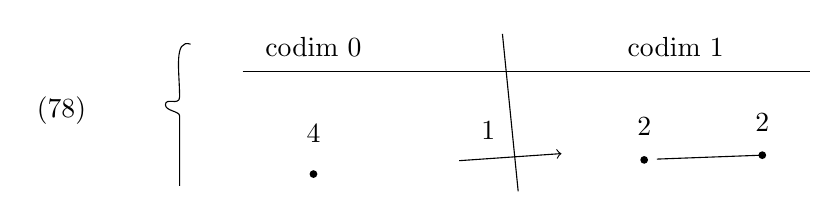
\begin{tikzpicture}[x=1cm,y=1cm]
\node at (-3.2,.8) {$(78)$};
\draw (-1.56,1.65) .. controls (-1.78,1.72) and (-1.70,1.30) .. (-1.70,.98) .. controls (-1.70,.86) and (-1.88,.98) .. (-1.88,.88) .. controls (-1.88,.80) and (-1.70,.80) .. (-1.70,.74) -- (-1.70,-.15);
\draw (-.9,1.30)--(6.3,1.30);
\draw (2.4,1.78)--(2.6,-.22);
\node at (0,1.62) {codim $0$};
\node at (4.6,1.62) {codim $1$};
\fill (0,0) circle (1.4pt);
\node[above] at (0,.28) {$4$};
\draw[->] (1.85,.17)--(3.15,.26);
\node[above] at (2.22,.31) {$1$};
\fill (4.2,.18) circle (1.4pt);
\fill (5.7,.24) circle (1.4pt);
\draw (4.36,.19)--(5.7,.24);
\node[above] at (4.2,.36) {$2$};
\node[above] at (5.7,.42) {$2$};
\end{tikzpicture}}
il n'y a plus qu'un seul pt à l'infini, correspondant aux trois p\textsuperscript{ts} à l'infini de $\widehat M^!_{0,4}$, permutés transitivement entre eux par $\mathfrak S_4$.

Caractéristiques d'EP fractionnaires. On trouve
\[
\begin{aligned}
\chi_!(M^{!\,\mathrm{an}}_{0,4})&=\chi_!(U^{\mathrm{an}}_{0,3})=2-2\underset{\substack{\Vert\\0}}{g}-\underset{\substack{\Vert\\3}}{\nu}=-1\\
\chi_!(\widehat M^{!\,\mathrm{an}}_{0,4})&=\chi_!(\mathbb P^{1\,\mathrm{an}})=2\\
\chi_!(\overset{\deleted{\unsure{\widehat{\phantom M}\,!}}}{M}{}^{\mathrm{an}}_{0,4})&=\chi_!(\unsure{U|\mathbb P}^{\mathrm{an}}_{0,3},\mathfrak S_4)\\
&=\chi_!\bigl(U^{\mathrm{an}}_{0,3}\smallsetminus\{-\bar j,-j\}\smallsetminus\{\tfrac12,2,-1\},\mathfrak S_4\bigr)\\
&\qquad+\chi_!(\{-\bar j,-j\},\mathfrak S_4)+\chi_!(\{\tfrac12,2,-1)\mathfrak S_4)\\
&=-1+\frac13+\frac12=-\frac1{\unsure{24|6}}
\end{aligned}
\]
\margin{\uline{NB} On peut écrire directement $\chi_!(U^{\mathrm{an}}_{0,3}):[\mathfrak S_4]=-\frac1{24}$}
\margin{61}

\scanpage{63}
\[
\chi_!(\widehat M^{\mathrm{an}}_{0,4})=\chi_!(\underbrace{U^{\mathrm{an}}_{0,3},\mathfrak S_4}_{-1/24})+\chi_!(\underbrace{\{0,1,\infty\},\mathfrak S_4}_{1/8})=\frac1{12}.
\]
De façon plus fine, dans un ``groupe de Grothendieck'' convenable, on aura
\margin{valable au dessus de $\mathbb Z[\frac16]$ --- \unsure{pour dispenser|pour me dispenser} de faire le calcul plus fin au dessus de $\operatorname{Spec}\mathbb Z\ldots$}
\[
79\quad\left\{\begin{aligned}
[M^!_{0,4}]&=[U_{\unsure{0,4|3,4}}]=\underbrace{T(1)}_{\substack{\text{``Tate''}\simeq[\mathbb E^1]\\(\text{d'augmentation }1)}}-2\\
[M_{0,4}]&=\deleted{\unsure{\tfrac1{24}(T(1)-2)}}\frac14(T(1)-2)+\frac1{12}+\frac18=\frac14(T(1)-1)-\frac1{24}\\
[\widehat M_{0,4}]&=[M_{0,4}]+\frac18=\deleted{\unsure{\tfrac1{24}(T(1)+1)}}=\frac14(T(1)-1)+\frac1{12}
\end{aligned}\right.
\]
Ces trois quantités sont d'augmentation égale resp\textsuperscript{t} : $-1,-1/24,1/12$.

$2^\circ)$ \uline{Cas \unsure{de|des}} $\widehat M_{1,1}$.
\diagram{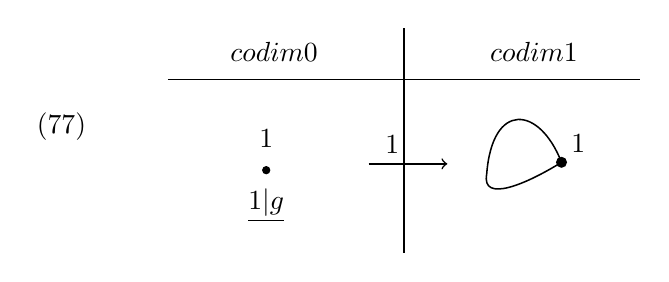
\begin{tikzpicture}[x=1cm,y=1cm,line width=.55pt]
\node at (-1.35,.55) {$(77)$};
\draw (0,1.15)--(6,1.15);
\draw (3,1.8)--(3,-1.05);
\node at (1.35,1.5) {$\text{codim }0$};
\node at (4.65,1.5) {$\text{codim }1$};
\fill (1.25,0) circle (1.5pt);
\node at (1.25,.4) {$1$};
\node at (1.25,-.45) {$\underline{\unsure{1|g}}$};
\draw[->] (2.55,.08)--(3.55,.08);
\node at (2.85,.32) {$1$};
\draw (5,.1)..controls(4.72,.82)and(4.12,.88)..(4.05,-.05)..controls(3.98,-.42)and(4.55,-.18)..(5,.1);
\fill (5,.1) circle (2pt);
\node[above right] at (5,.1) {$1$};
\end{tikzpicture}}
Il y a exactement un point à l'infini.

On a un morphisme (\uline{au dessus de} $\mathbb Z[\frac12]$)
\[
(78)\qquad \overset{\deleted{\unsure{\wedge}}}{M}_{1,1}\longrightarrow\overset{\deleted{\unsure{\wedge}}}{M}'_{1,4}\overset{\mathrm{déf}}{=}(\overset{\deleted{\unsure{\wedge}}}{M}^!_{1,4},\mathfrak S_3)
\]
qui fait de $\overset{\deleted{\unsure{\wedge}}}{M}_{1,1}$ une gerbe (de groupe constant $\{\pm1\}$) au dessus de $\overset{\deleted{\unsure{\wedge}}}{M}'_{1,4}$ (en ca. $\neq2$)
\[
\text{d'où}\qquad [M_{1,1}]=\frac12[U_{0,3},\mathfrak S_3]=\unsure{2|\frac12}[M_{0,4}]\underset{\inserted{T(1)}}{\deleted{\unsure{=\tfrac1{12}[\mathbb E^1]-\tfrac14}}}
\]
\margin{62}

\scanpage{64}
\mspage{31}
d'où, au moins au dessus de $\mathbb Z[\frac12]$
\[
(79)\quad\left\{\begin{aligned}
[M_{1,1}]&=\deleted{\unsure{\tfrac1{12}(T(1)-2)}}\frac12(T(1)-1)-\frac1{12}\\
[\widehat M_{1,1}]&=[M_{1,1}]+\underset{\substack{\Vert\\1/2}}{[\widehat M^\infty_{1,1}]}=\deleted{\unsure{\tfrac{T(1)}{12}+\tfrac13}}\frac12(T(1)-1)+\frac5{12}
\end{aligned}\right.
\]
Voici un autre calcul de $[M_{1,1}]$. On considère le morphisme modulaire
\[
M_{1,1}\longrightarrow\mathbb E^1
\]
\deleted{et} en découpant $\mathbb E^1$ suivant les deux sections $S_0$ (correspondant à la courbe elliptique harmonique de groupe d'\unsure{automs|autos} $\mathbb Z/4\mathbb Z$) et $S_{\deleted{\unsure{0}}1}$ \deleted{\unsure{$\simeq\mathbf Z$}} (courbe ell. \unsure{bonne} \unsure{avec un bon} gr. d'\unsure{automs|autos} $\mathbb Z/6\mathbb Z$), qui ne se coupent qu'en les pts $2$ et $3$, qui correspondent (sauf erreur) à des groupes d'\unsure{automs|autos} d'ordre $24$, et $12$. On a donc une partition
\[
\mathbb E^1=\deleted{\unsure{\mathbb E}}U\amalg S'_0\amalg S'_1\cup a_2\cup a_3
\]
où \deleted{\unsure{$a_1,a_0$}}
\[
\begin{gathered}
U=\mathbb E^1\unsure{+|\smallsetminus}(S_0\cup S_1)\\
\left\{\begin{aligned}
\{\underset{\substack{|\\\text{car }2}}{a_2},\underset{\substack{|\\\text{car. }3}}{a_3}\}&=S_0\cap S_1\\
S'_0&=S_0\smallsetminus\{a_{\unsure{2|3}},a_3\},\quad S'_1=S_1\smallsetminus\{a_2,a_3\}
\end{aligned}\right.
\end{gathered}
\]
On trouve donc
\margin{63}

\scanpage{65}
\[
M_{1,1}=\frac12[U]+\frac14[S'_0]+\frac16[S'_1]+\frac1{24}[a_2]+\frac1{12}[a_3]
\]
et on a
\[
\begin{aligned}
[U]&=[\mathbb E^1]-[S_0]-[S_1]+[a_2]+[a_3]\\
&=T(1)-2+\zeta_2+\zeta_3
\end{aligned}
\]
où de façon générale on pose, pour un nb premier $p$
\[
\zeta_p=[\operatorname{Spec}\mathbb Z/p\mathbb Z]=i_{p!}(1)
\]
où
\[
i_{p!}:K_!(\mathbb Z_p)\unsure{\longrightarrow} K_!(\mathbb Z).
\]
De $=$
\[
\begin{aligned}
[S'_0]&=[S_0]-[a_2]-[a_3]=1-\zeta_2-\zeta_3\\
[S'_1]&=[S_1]-[a_2]-[a_3]=1-\zeta_2-\zeta_3
\end{aligned}
\]
d'où
\[
\begin{aligned}
[M_{1,1}]&=\frac12(T(1)-2+\zeta_2\unsure{-|+}\zeta_3)+\overbrace{\left(\frac14\deleted{\unsure{4|+}}+\frac16\right)}^{5/12}(1-\zeta_2-\zeta_3)\\
&\qquad+\frac1{24}\zeta_2+\frac1{12}\zeta_3\\
&=\frac12T(1)-7/12\deleted{\unsure{\zeta|4}}+\unsure{\frac18}\zeta_2+\frac16\zeta_3\\
&=\frac12(T(1)-1)-\frac1{12}+\frac18\zeta_2+\frac16\zeta_3,
\end{aligned}
\]
donc
\[
(80)\quad\left\{\begin{aligned}
[M_{1,1}]&=\frac12(T(1)-1)-\frac1{12}+\frac18\zeta_2+\frac16\zeta_3\\
[\widehat M_{1,1}]&=[M_{1,1}]+\frac12=\frac12T(1)-\frac1{12}+\frac18\zeta_2+\frac16\zeta_3
\end{aligned}\right.
\]
\margin{64}

\scanpage{66}
\mspage{32}
$3^\circ)$ \uline{Cas \unsure{de|des}} $\widehat M^!_{0,5}$, ou $\widehat M_{0,I}$
\diagram{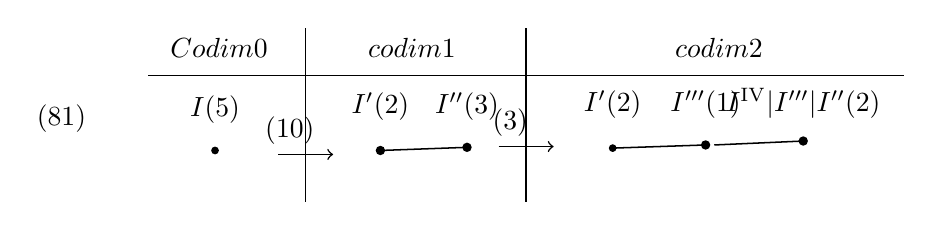
\begin{tikzpicture}[x=1cm,y=1cm,line width=.55pt]
\node at (-1.1,.4) {$(81)$};
\draw (0,.95)--(9.6,.95);
\draw (2,1.55)--(2,-.65);
\draw (4.8,1.55)--(4.8,-.65);
\node at (.9,1.3) {$\text{Codim }0$};
\node at (3.35,1.3) {$\text{codim }1$};
\node at (7.25,1.3) {$\text{codim }2$};
\fill (.85,0) circle (1.4pt);
\node[above] at (.85,.22) {$I(5)$};
\draw[->] (1.65,-.05)--(2.35,-.05);
\node[above] at (1.8,-.05) {$(10)$};
\draw (2.95,0)--(4.05,.04);
\fill (2.95,0) circle (1.7pt);
\fill (4.05,.04) circle (1.7pt);
\node[above] at (2.95,.26) {$I'(2)$};
\node[above] at (4.05,.26) {$I''(3)$};
\draw[->] (4.45,.05)--(5.15,.05);
\node[above] at (4.6,.05) {$(3)$};
\draw (5.9,.03)--(7.08,.07);
\draw (7.19,.07)--(8.32,.12);
\fill (5.9,.03) circle (1.4pt);
\fill (7.08,.07) circle (1.7pt);
\fill (8.32,.12) circle (1.7pt);
\node[above] at (5.9,.28) {$I'(2)$};
\node[above] at (7.08,.28) {$I'''(1)$};
\node[above] at (8.32,.28) {$\unsure{I^{\mathrm{IV}}|I'''|I''}(2)$};
\end{tikzpicture}}
Dans \unsure{de|le} $\widehat M^!_{0,5}$ il y a dix ``diviseurs à l'infini'', dont chacun est un $\widehat M^!_{0,4}$ \deleted{\unsure{$\simeq\mathbb P$}}, \deleted{\unsure{$\mathbb P^1_{0,3}\mathfrak S_3$}} \inserted{(plus précisément, un $\widehat M_{0,I''(3)\amalg(*)}\simeq(\mathbb P^1_{I''})_{\mathbb Z}$)} (ayant comme on avait vu, et \unsure{avait|aurait}) trois points à l'infini --- les pts à l'infini sont en nb total $\frac{30}{2}=15$, correspondant aux partitions de $I(5)$ de type $(2,2,1)$, alors que les diviseurs à l'infini correspondent aux parties \inserted{$I'$} de $I$ de cardinal $2$. Deux tels diviseurs, correspondant à des parties $I',I''\in\mathfrak P_2(I)$, se rencontrent sss \deleted{elles} on a $I'\cap I''=\phi$, i.e. \unsure{sss|\deleted{sss}} $I',I''$ et $I\smallsetminus(I'\cup I'')$ forment justement une partition de $I$ de type $(2,2,1)$.
\margin{$\mathbb P^1_{I''}\overset{\mathrm{def}}{=}\mathbb P^1_{\mathbb Z}\wedge_{\mathfrak S_3}\operatorname{Isom}(\{0,1,\infty\},I'')$}

D'après l'étude combinatoire de l'icosaèdre, \unsure{choisissant|choisissons} une orientation de $I$ --- ce qui détermine un icosaèdre orienté, ou encore un icos. gauche) les $10$ diviseurs à l'infini \deleted{\unsure{en ordre}} de $\widehat M_{0,I}$, i.e. les \inserted{$10$} \unsure{elmts|elts} de $\mathfrak P_2(I)$, \inserted{ou (par} \deleted{\unsure{correspon-}}
\margin{65}

\scanpage{67}
passage aux complémentaires) les dix ``triangles'' de $I$, \unsure{correspondant|correspondent} aux dix faces de l'icosaèdre gauche ($\simeq$ paires de faces opposées de l'icos. ordinaire), tandis que les $15$ partitions de type $(2,2,1)$ de $I$, qu'on peut interpréter comme les structures carrées sur quatre parmi les $5$ pts de $I$
\figure{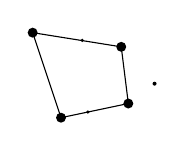
\begin{tikzpicture}[scale=.9]\draw (0,1.1)--(1.25,.9)--(1.35,.1)--(.4,-.1)--cycle;\foreach \p in {(0,1.1),(1.25,.9),(1.35,.1),(.4,-.1)}{\fill \p circle (2pt);}\fill (.7,.99) circle (.7pt);\fill (.78,-.02) circle (.7pt);\fill (1.72,.38) circle (.8pt);\end{tikzpicture}}
(en associant à un tel carré les deux paires de sommets diagonalement opposés) correspondent aux $15$ arêtes dudit icosaèdre gauche.
\margin{NB on associe à un côté $a$ le jeu des ``couleurs'' des $4$ autres côtés des faces \deleted{\unsure{deux}} adjacentes, groupées \deleted{\unsure{deux}} \unsure{en} deux paires \unsure{des deux faces}
\figure{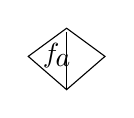
\begin{tikzpicture}[scale=.65]\draw (0,0)--(.75,.55)--(1.5,0)--(.75,-.65)--cycle;\draw (.75,.48)--(.75,-.65);\node at (.45,.02) {$f$};\node at (.68,-.08) {$a$};\end{tikzpicture}}}
Un côté \inserted{$a$} est contenu \deleted{dans}\inserted{(\uline{incident})} à une face \inserted{$f$} de l'icosaèdre, sss le ``triangle'' $\subset I$ correspondant à $f$ a comme intersection avec le carré correspondant à $a$, \unsure{\deleted{deux}\inserted{l'un des}|\inserted{l'un des} deux} \deleted{\unsure{côt}} $2$ sommets \deleted{consécutifs}\inserted{opposés} du carré, \deleted{On voit donc.}\inserted{i.e. ssi le complémentaire du triangle est formé de l'une des deux paires définissant le carré.}
\inserted{Donc on voit que} la relation d'incidence des diviseurs à sommets de la structure $\widehat M_{0,I}$, correspond \unsure{à|:} celle des faces et arêtes de l'icosaèdre gauche, ou par dualité, à celle des \deleted{arêtes}\inserted{sommets} et des \deleted{faces}\inserted{arêtes} du dodécaèdre.

On a donc trouvé :
\margin{66}

\scanpage{68}
\mspage{33}
\uline{Proposition} Le diviseur à l'infini \inserted{$M^\infty_{0,I}$} de $\widehat M_{0,I}$ est une courbe standart \inserted{\unsure{déployé|déployée}} sur $\operatorname{Spec}\mathbb Z$, dont le graphe est isomorphe au \deleted{celui du} $1$-squelette du dodécaèdre gauche défini par $I$ (muni d'une orientation convenable).
\margin{\uline{NB} $\widehat M_{0,I}\longrightarrow$ un vrai schéma projectif et lisse \unsure{et tout|et tant} --- le groupoïde qu'il représente est en effet rigide. Il en \unsure{va} pour tous les $M_{0,I}\simeq M^!_{0,\nu}$ quelque soit $\nu\in\mathbb N\ldots$}

Bien entendu, les genres des comp. irréductibles sont nuls, Il n'y a pas \inserted{lieu de mettre} des ``pts marqués'' sur \deleted{\unsure{$M_{0,I}$}} les \inserted{$10$} composantes irréductibles de $M^\infty_{0,I}$, qui est de toutes façons une MD-courbe \deleted{\unsure{stable}} à MD-graphe maximal (tous les genres nuls, tous les sommets d'ordre $3$, pas de pieds marqués).

L'isom. de la prop. précédente tient compte des opérations de $\mathfrak S_I^+$ \inserted{$\simeq\operatorname{Aut}\text{ du dodécaèdre gauche}$} sur $M^\infty_{0,I}$, mais pas de celles de $\mathfrak S_I$ \deleted{\unsure{tout}} entier --- il faudrait le comprendre du pt de vue de la géométrie de l'icosaèdre \inserted{gauche} (ou du dodécaèdre \inserted{gauche}\ldots) --- ça doit être lié bien sûr au \uline{bi-icosaèdre} gauche combinatoire\unsure{)|]}

Quand on passe à la multiplicité modulaire
\margin{67}

\scanpage{70}
\mspage{34}
$4^\circ)$ \uline{Cas de} $\widehat M^!_{1,2}\simeq\widehat M^{\deleted{\unsure{!}}}_{1,I}$ $(\operatorname{card}I=2\deleted{\unsure{\}}},\ I=\{a,b\})$
\diagram{\begin{tikzcd}[ampersand replacement=\&,column sep=18pt,row sep=28pt,
execute at end picture={
\draw ([xshift=9pt]scan070-codim-zero.east |- scan070-codim-zero.north) -- ([xshift=9pt,yshift=-10pt]scan070-codim-zero.east |- scan070-g-one.south);
\draw ([xshift=-9pt]scan070-p-one.west |- scan070-codim-zero.north) -- ([xshift=-9pt,yshift=-12pt]scan070-p-one.west |- scan070-p-one.south);
\path (scan070-g-zero.center) -- (scan070-g-one.center) coordinate[midway] (scan070-middle);
\node at (scan070-codim-zero.center |- scan070-middle) {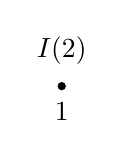
\begin{tikzpicture}[baseline=-2pt]\fill(0,0)circle(1.5pt);\node[above]at(0,.15){$I(2)$};\node[below]at(0,-.08){$1$};\end{tikzpicture}};
\coordinate (scan070-brace-top) at ([xshift=-18pt,yshift=2pt]scan070-codim-zero.north west);
\coordinate (scan070-brace-bottom) at ([xshift=-18pt]scan070-codim-zero.west |- scan070-g-one.center);
\path (scan070-brace-top) -- (scan070-brace-bottom) coordinate[midway] (scan070-brace-middle);
\draw (scan070-brace-top) .. controls ([xshift=-5pt]scan070-brace-top) and ([xshift=-2pt,yshift=4pt]scan070-brace-middle) .. ([xshift=-9pt]scan070-brace-middle) .. controls ([xshift=-2pt,yshift=-4pt]scan070-brace-middle) and ([xshift=-5pt]scan070-brace-bottom) .. (scan070-brace-bottom);
\node[left=5pt]at([xshift=-9pt]scan070-brace-middle){$(83)$};
}]
|[alias=scan070-codim-zero]|\text{codim }0\&\text{codim }1\&\text{codim }2\\
\&|[alias=scan070-g-zero]|G_0=\text{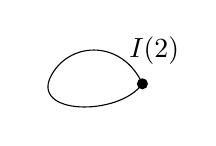
\begin{tikzpicture}[baseline=-2pt]\draw(0,0)..controls(-.25,.55)and(-.9,.55)..(-1.15,.12)..controls(-1.45,-.4)and(-.3,-.42)..(0,0);\fill(0,0)circle(2pt);\node[above]at(.15,.12){$I(2)$};\end{tikzpicture}}\arrow[r,"2"]\arrow[dr,"1"']\&
\text{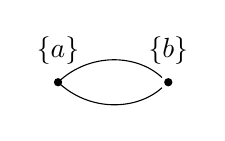
\begin{tikzpicture}[baseline=-2pt]\draw(0,0)..controls(.4,.38)and(1,.36)..(1.32,.06);\draw(0,0)..controls(.4,-.38)and(1,-.36)..(1.32,-.07);\fill(0,0)circle(1.5pt);\fill(1.4,0)circle(1.5pt);\node[above]at(0,.1){$\{a\}$};\node[above]at(1.4,.1){$\{b\}$};\end{tikzpicture}}=P_0\\
\&|[alias=scan070-g-one]|G_1=\text{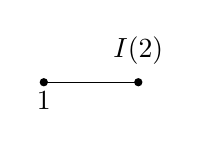
\begin{tikzpicture}[baseline=-2pt]\draw(0,0)--(1.2,0);\fill(0,0)circle(1.5pt);\fill(1.2,0)circle(1.5pt);\node[below]at(0,0){$1$};\node[above]at(1.2,.1){$I(2)$};\end{tikzpicture}}\arrow[r,"1"]\&
|[alias=scan070-p-one]|\text{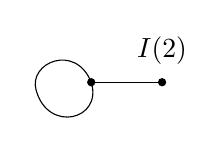
\begin{tikzpicture}[baseline=-2pt]\draw(0,0)..controls(-.2,.5)and(-.8,.25)..(-.7,-.1)..controls(-.55,-.65)and(.15,-.48)..(0,0);\draw(0,0)--(.9,0);\fill(0,0)circle(1.5pt);\fill(.9,0)circle(1.5pt);\node[above]at(.9,.1){$I(2)$};\end{tikzpicture}}=P_1
\end{tikzcd}}
\margin{$D_{\begin{tikzpicture}[x=1ex,y=1ex,baseline=-.2ex,line width=.3pt]\draw (0,0)..controls(-.35,.25)and(-.9,.3)..(-.95,0)..controls(-.9,-.3)and(-.35,-.25)..(0,0);\fill(0,0)circle(.6pt);\end{tikzpicture}}$ ``D boucle''\quad $D_{\bullet-\bullet}$ ``D segment''}
Il y a deux diviseurs à l'infini, \inserted{$D_{\begin{tikzpicture}[x=1ex,y=1ex,baseline=-.2ex,line width=.3pt]\draw (0,0)..controls(-.35,.25)and(-.9,.3)..(-.95,0)..controls(-.9,-.3)and(-.35,-.25)..(0,0);\fill(0,0)circle(.6pt);\end{tikzpicture}}$ et $D_{\bullet-\bullet}$,} et deux points \inserted{critiques} à l'infini, \deleted{dont}\inserted{$P_0$ et $P_1$,} l'un \inserted{$P_0$} est contenu dans $D_{\begin{tikzpicture}[x=1ex,y=1ex,baseline=-.2ex,line width=.3pt]\draw (0,0)..controls(-.35,.25)and(-.9,.3)..(-.95,0)..controls(-.9,-.3)and(-.35,-.25)..(0,0);\fill(0,0)circle(.6pt);\end{tikzpicture}}$ et dans $D_{\bullet-\bullet}$, et l'autre n'est contenu que dans $D_{\bullet-\bullet}$.

Essayons de \inserted{bien} saisir la structure de la multiplicité schématique à l'infini $\widehat M^\infty_{1,I}\simeq\widehat M^{!\,\infty}_{1,2}$, qui est la réunion amalgamée des deux multiplicités lisses \deleted{\unsure{$\widehat M$}} $D_{\begin{tikzpicture}[x=1ex,y=1ex,baseline=-.2ex,line width=.3pt]\draw (0,0)..controls(-.35,.25)and(-.9,.3)..(-.95,0)..controls(-.9,-.3)and(-.35,-.25)..(0,0);\fill(0,0)circle(.6pt);\end{tikzpicture}}$ et $D_{\bullet-\bullet}$.
$D_{\begin{tikzpicture}[x=1ex,y=1ex,baseline=-.2ex,line width=.3pt]\draw (0,0)..controls(-.35,.25)and(-.9,.3)..(-.95,0)..controls(-.9,-.3)and(-.35,-.25)..(0,0);\fill(0,0)circle(.6pt);\end{tikzpicture}}$ est isomorphe à $(\widehat M^{\unsure{!}}_{G_0},\Gamma^!_0)$, où $G_0$ est le \inserted{MD-}graphe
\figure{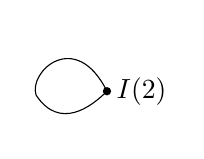
\begin{tikzpicture}[baseline=-2pt]\draw (0,0)..controls(-.4,.8)and(-1,.25)..(-.9,-.05)..controls(-.6,-.5)and(-.2,-.2)..(0,0);\fill(0,0)circle(1.5pt);\node[right]at(0,0){$I(2)$};\end{tikzpicture}},
$\Gamma_0$ son groupe d'automorphismes, et $\Gamma^!_0=\operatorname{Ker}(\Gamma_0\longrightarrow\mathfrak S_{I(G_0)})\simeq\mathbb Z/2$
D'ailleurs $\widehat M_{G_0}\simeq\widehat M^!_{0,4}\simeq\mathbb P^1_{\mathbb Z}$, sur lequel $\Gamma^!_0\simeq\mathbb Z/2$ opère en fixant un des \inserted{trois} pts à l'infini de $U_{0,3\,\mathbb Z}$, \inserted{soit $1$,} et en transposant les deux autres, \inserted{soit $\{0,\infty\}$,} \deleted{De \unsure{façon} plus \unsure{intrinsèque},} \inserted{(Ceci correspond au} choix d'un élément de $I$ comme $\unsure{1|\underline 1}$, et les deux éléments de $\widetilde A(G_0)$ comme $0$ et $\infty$ !) donc on trouve en ``quotient'' par $z\longmapsto z^{-1}$. De façon
\margin{69}

\scanpage{71}
plus intrinsèque, le graphe $G_0$ \deleted{\unsure{se déploie}} associe à l'ens $I\amalg\widetilde A'_0$ de card $4$, muni d'une partition de type $(2,2)$ (et $=$ d'une partie \inserted{$I$} de card $2$), l'ens \inserted{$J$} des \inserted{$3$} partitions de type $(2,2)$ a donc un pt marqué $\varepsilon_1$, les deux autres pts correspondent aux élts de l'ens $\unsure{J':|J^!}=I\wedge_{\mathbb Z/2}\widetilde A'_0$ :
\[
(\unsure{84|83})\qquad J=\{\varepsilon_1\}\amalg J'\qquad J'=I\wedge_{\mathbb Z/2}\widetilde A'_0.
\]
Ceci posé, $\mathbb P^1_J=\mathbb P^1_{\{\varepsilon_1\}\amalg J'}\deleted{\unsure{\mathfrak S_{J'}}}$ peut être considéré comme le compactifié de $\mathbb G_m^{1}\wedge_{\pm1}J'$ et \deleted{$\unsure{\mathfrak S_2}$} $\mathfrak S_{J'}\simeq\mathbb Z/2$ y opère par transfert de structure. On a.
\margin{$\varepsilon_1$ correspond au point $1$}
\[
(85)\qquad
\left\{\begin{aligned}
\widehat M_{G_0}&\simeq(\mathbb P^1_{\{\varepsilon_1\}\amalg J'}\deleted{\unsure{\mathfrak S_{J'}}})\\
(\widehat M_{G_0},\Gamma^!_0)&\simeq(\mathbb P^1_{(\varepsilon_1\amalg J')},\mathfrak S_{J'})
\end{aligned}\right.
\]
\margin{$(\unsure{\widehat M_{D_0\bar\varepsilon}})$}
sur lesquels $\mathfrak S_I$ opère via $\mathfrak S_{J'}$, donc $\mathfrak S_I$ \uline{opère trivialt sur} $\widehat M_{D_0}$. Les deux pts à l'infini de $\widehat M_{D_0}$ correspondent : la trajectoire $J'$ d'une part \inserted{(pt. $P_0$)}\unsure{:|;|à} la trajectoire $\varepsilon_1$ d'autre part (point $P_1$). On a
\[
(86)\qquad M_{D_0}\simeq\mathbb E^1_{\mathbb Z}\setminus\{\text{section }2\}=\operatorname{Spec}\mathbb Z[T]_{(T-2)}
\]
\[
\text{via}\quad\left\{\begin{aligned}M_{G_0}&\longrightarrow M_{D_0}\\ T&\longrightarrow T+\frac1T\end{aligned}\right.
\]
\[
(87)\qquad\widehat M_{D_0}\simeq\bigl(\mathbb P^1_{\mathbb Z},\text{ avec ``signature'' }2\text{ le long de la section }T=2\bigr)
\]
\margin{70}

\scanpage{72}
\mspage{35}
dans ce dernier iso, $P_0$ correspond à la section à l'infini, et $P_1$ à la section $2$ de $\mathbb P^1_{\mathbb Z}$.

D'autre part, on a
\[
(88)\qquad \widehat M_{D_1}\unsure{=|\simeq}\widehat M_{G_1}\simeq\widehat M_{1,1}
\deleted{\simeq\bigl(\mathbb P^1_{\mathbb Z},\text{ avec signatures }4\text{ et }6\text{ le long des sections }0\text{ et }\unsure{J_1|j_1}=2^{\unsure{\alpha}}3^{\unsure{\beta}}\text{ (correspond. à la courbe elliptique d'autom }\unsure{\mathbb Z/4\mathbb Z|\mathbb Z/6\mathbb Z}\bigr)}
\]
\deleted{dans le dernier iso, \inserted{\deleted{\unsure{lorsque}}} la section à \unsure{l'infini} de $\widehat M_{D_1}$}

Je me rends compte qu'il me faudrait mieux comprendre la structure de $\widehat M_{1,1}$ (et $=$ de $M_{1,1}$), à commencer dans le cadre transcendant (analytique complexe, avec évt. la structure réelle \unsure{explicite} -- i.e. considération de la conjugaison complexe\ldots). J'y reviendrai plus loin.

\uline{Notons déjà}

\uline{Proposition} Si $\dim M_G\geq2$, alors $M_G^\infty$ est \inserted{\unsure{géom.}} connexe \inserted{(fibre par fibre)}.

Dém. Écrivons
\[
(89)\qquad\left\{\begin{aligned}
\widehat M_G&\simeq\prod_{\alpha\in S}\widehat M^{!}_{g_\alpha,\widehat\nu_\alpha}\\
M_G&\simeq\prod_{\alpha\in S}\overset{\deleted{\unsure{\wedge}}}{M}^{!}_{g_\alpha,\widehat\nu_\alpha}
\end{aligned}\right.
\]
\margin{71}

\scanpage{73}
et utilisant le fait que les $\widehat M^{!}_{g_\alpha,\widehat\nu_\alpha}$ sont
connexes, on voit que $\overset{\unsure{\deleted{\wedge}|\sim}}{M}_G^\infty=\widehat M_G\setminus M_G$
est connexe dès que \deleted{\unsure{deux}} parmi les
facteurs $\widehat M^{!}_{g_\alpha,\widehat\nu_\alpha}$, il y en a au moins
deux qui sont de dim $\geq1$ (en utilisant
le fait que pour un tel $\alpha$, on a
$M^\infty_{g_\alpha,\widehat\nu_\alpha}\ne\phi$). Donc il suffit de regarder
le cas où $\widehat M_G\simeq\widehat M^{!}_{g,\nu}\inserted{\simeq \unsure{\widehat M_{g,I}|M_{g,I}}}$, avec
\inserted{le cas où $\unsure{3g-1)+\nu=2|3(g-1)+\nu=2}$ est déjà vu, donc DPS $N\geq3$.}
\inserted{$(\dim M_{g,\nu}=)$} $N=\unsure{2|3}\unsure{(}g-1)+\nu\geq2$.
\deleted{Dans ce cas}, Il suffit de
voir que deux diviseurs à l'infini peuvent
être joints par une chaine de tels div.
dont deux consécutifs ont une intersection
non vide, compte tenu que ces diviseurs
sont eux aussi connexes. Or les diviseurs
à l'infini correspondent aux \deleted{types} \inserted{MD-}graphes
suivants
\figure{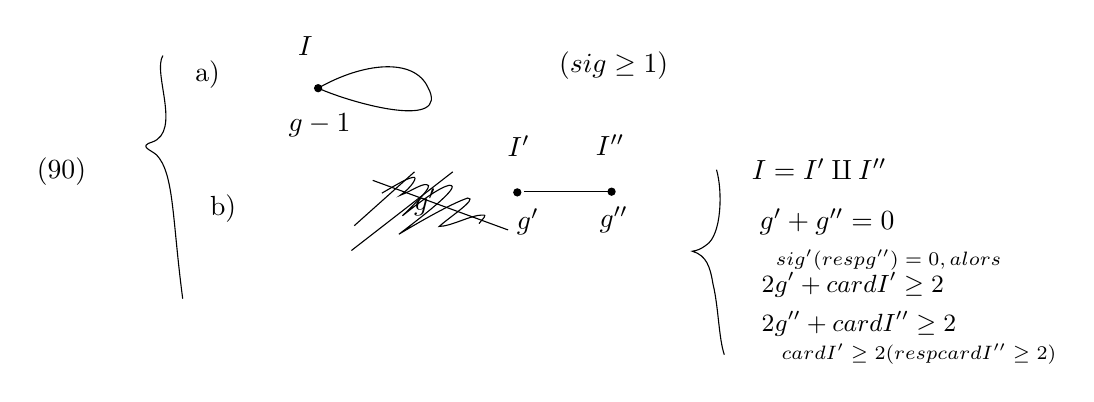
\begin{tikzpicture}[x=.009cm,y=-.009cm]
\node at (47,207) {$(90)$};
\draw (190,43)..controls(175,67)and(217,150)..(175,165)..controls(155,171)and(173,176)..(181,183)..controls(206,209)and(203,273)..(218,386);
\node at (253,70) {a)};
\fill(409,89)circle(1.5pt);
\draw(409,89)..controls(472,53)and(544,45)..(564,88)..controls(596,148)and(461,112)..(409,89);
\node at (391,30) {$I$};
\node at (411,142) {$g-1$};
\node at (826,57) {$(\text{si }g\geq1)$};
\node at (275,259) {b)};
\node at (560,250) {\deleted{$\unsure{g'}$}};
\draw (460,283)--(545,207);
\draw (499,237)..controls(515,228)and(532,217)..(542,215)..controls(552,212)and(540,230)..(525,240)..controls(541,234)and(554,224)..(562,225)..controls(575,225)and(540,257)..(528,269)..controls(548,253)and(579,229)..(594,226)..controls(615,225)and(552,273)..(523,295)..controls(548,280)and(596,252)..(620,244)..controls(636,244)and(590,274)..(580,284)..controls(596,284)and(625,268)..(640,268)..controls(650,267)and(640,274)..(636,280);
\draw (456,318)--(599,207);
\draw (486,219)--(677,289);
\fill(690,236)circle(1.5pt);
\draw(700,235)--(823,235);
\fill(823,235)circle(1.5pt);
\node at (692,171) {$I'$};
\node at (821,170) {$I''$};
\node at (705,278) {$g'$};
\node at (826,275) {$g''$};
\draw(971,204)..controls(980,235)and(978,296)..(957,310)..controls(949,316)and(944,318)..(937,319)..controls(957,325)and(962,341)..(966,365)..controls(974,398)and(974,441)..(982,465);
\node[anchor=base west] at (1007,218) {$I=I'\amalg I''$};
\node[anchor=base west] at (1018,289) {$g'+g''=0$};
\node[anchor=base west,font=\scriptsize] at (1041,339) {$\inserted{\text{si }g'\text{ (resp }g'')=0,\text{ alors}}$};
\node[anchor=base west,font=\small] at (1021,377) {$\deleted{2g'+\operatorname{card}I^{\unsure{\prime}}\geq\unsure{2}}$};
\node[anchor=base west,font=\small] at (1021,432) {$\deleted{2g''+\operatorname{card}I''\geq2}$};
\node[anchor=base west,font=\scriptsize] at (1049,472) {$\inserted{\operatorname{card}I'\geq2\text{ (resp }\operatorname{card}I''\geq2\text{)}}$};
\end{tikzpicture}}
\margin{72}

\scanpage{74}
\mspage{36}
On a comme spécialisation du cas a)
\figure{\begin{tikzpicture}[x=1cm,y=1cm]
\node at (-1,.1) {$(91)$}; \node at (0,.3) {$a'$)};
\node at (-.25,.8) {$\unsure{\deleted{b}|b}$};
\fill (2,.2) circle (1.4pt); \fill (4,.2) circle (1.4pt);
\draw (2,.2)..controls (1.25,1.1) and (.25,.6)..(.6,-.1)..controls (.8,-.65) and (1.6,-.1)..(2,.2);
\draw (2.17,.2)--(4,.2); \draw (2.1,.35)..controls (2.8,.55) and (3.6,.55)..(3.9,.3);
\foreach \x in {2.2,2.35,...,3.8}{\draw (\x,.37)--(\x+.12,.5);}
\node[above] at (2,.65) {$I_1$};\node[below] at (2,.1) {$g_1$};
\node[above] at (4,.65) {$I_2$};\node[below] at (4,.1) {$g_2$};
\node[anchor=west,align=left] at (5.5,.15) {$\begin{gathered}I_1\amalg I_2=I\\g_1+g_2=g-1\\\text{si }g_2=0\quad\deleted{\unsure{quelconque}}\ \inserted{\text{on a }\operatorname{card}I_2\geq2}\\\deleted{\unsure{\text{on a }I_1\ne\phi\text{ (et card }I_2\ne\phi\text{)}}}\end{gathered}$};
\end{tikzpicture}}
\margin{NB OPS $g_2=1$, $g_1=g-2$\\pourvu que $g\geq2$\\$(I_1,I_2)$ partition quelc. de $I$}
On a comme spécialisation du cas b), \deleted{\unsure{si on suppose} $g'$}
\figure{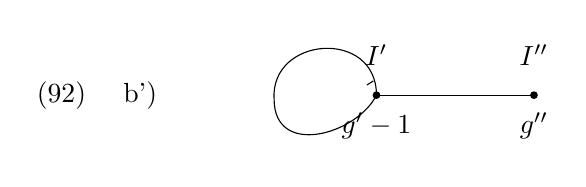
\begin{tikzpicture}[x=1cm,y=1cm]
\node at (-1,0) {$(92)$};\node at (0,0) {b')};
\fill (3,0) circle (1.4pt);\fill (5,0) circle (1.4pt);\draw (3,0)--(5,0);
\draw (3,0)..controls (3,.85) and (1.65,.75)..(1.7,-.05)..controls (1.7,-.8) and (2.75,-.5)..(3,0);
\draw (2.96,.18)--(2.88,.13);
\node[above] at (3,.25) {$I'$};\node[below] at (3,-.1) {$g'-1$};
\node[above] at (5,.25) {$I''$};\node[below] at (5,-.1) {$g''$};
\end{tikzpicture}}
Donc si $g\geq1$ (de sorte que le cas a) existe) alors prenant dans b) \deleted{\unsure{avec} $g'\ne$} les \unsure{notations} $g',g''$ de sorte que $g'\ne0$ i.e. $g'\geq1$ (quitte à éch. \deleted{$\unsure{g}$} $g',g''$), on voit que l'on a une spécialisation \inserted{b') $=$ a')} commune aux cas a) et b). Cela démontre notre assertion lorsque $g\ne0$. \deleted{Si $g$} Dans le cas $g=0$, \inserted{donc $\operatorname{card}I\geq6$} il n'y a que les cas b), \deleted{et \unsure{OPS}} \deleted{\unsure{a il y a}} \inserted{Or on a} \deleted{\unsure{pour} $\operatorname{card}I'\unsure{\geq|>}\operatorname{card}I''$, donc $\operatorname{card}I'\geq3$\unsure{;|,} \unsure{qui a donc} la spécialisation} une spécialisation de la forme
\figure{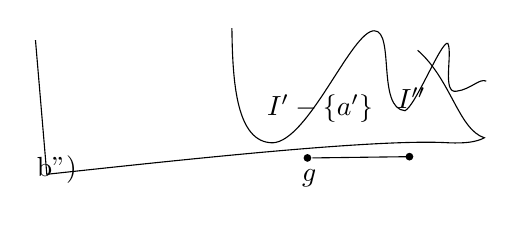
\begin{tikzpicture}[x=.008cm,y=-.008cm]
\node at (52,243) {\deleted{b'')}};
\node at (470,147) {\deleted{$I'-\{a'\}$}};
\node at (615,130) {\deleted{$I''$}};
\fill (450,225) circle (1.4pt); \fill (612,223) circle (1.4pt);
\draw (458,225)--(612,223);
\node at (453,258) {\deleted{$\unsure{g}$}};
\draw (18,38)--(36,251)
 ..controls (250,228) and (560,194)..(675,201)
 ..controls (700,202) and (718,200)..(731,193)
 ..controls (690,180) and (678,100)..(625,54);
\draw (330,19)
 ..controls (331,105) and (337,201)..(395,201)
 ..controls (452,198) and (520,23)..(556,23)
 ..controls (589,23) and (560,147)..(605,150)
 ..controls (622,142) and (663,38)..(673,43)
 ..controls (681,60) and (663,124)..(687,119)
 ..controls (710,116) and (723,98)..(734,103);
\end{tikzpicture}}
\figure{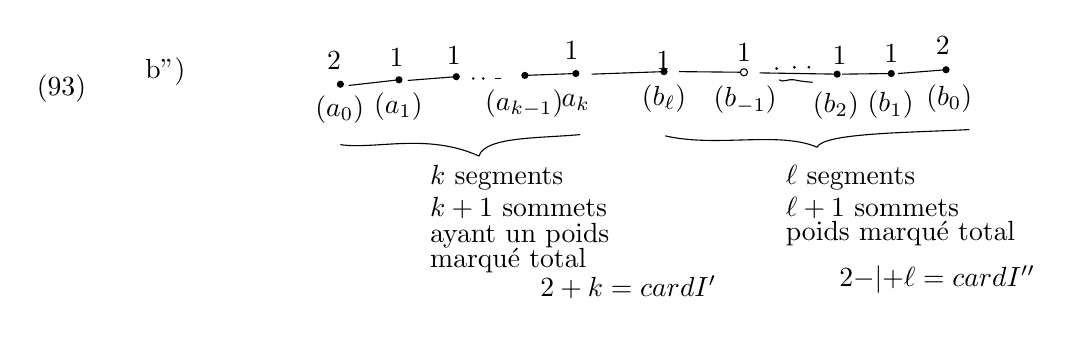
\begin{tikzpicture}[x=.008cm,y=-.008cm]
\node at (40,87) {$(93)$}; \node at (205,60) {b'')};
\draw (496,82)--(576,73) (590,74)--(667,68)
 (776,66)--(857,63) (882,64)--(997,60)
 (1021,60)--(1124,61) (1149,62)--(1272,64)
 (1280,64)--(1358,63) (1369,63)--(1445,57);
\fill (694,71) circle (.5pt); \fill (710,71) circle (.5pt);
\draw (728,71)--(738,71);
\fill (1176,55) circle (.55pt); \fill (1204,53) circle (.55pt);
\fill (1227,53) circle (.55pt);
\draw (1180,73)..controls (1185,78) and (1195,71)..(1204,73)
 ..controls (1217,76) and (1225,76)..(1233,77);
\foreach \x/\y in {483/80,576/73,667/68,776/66,857/63,997/60,1272/64,1358/63,1445/57}
 {\fill (\x,\y) circle (1.3pt);}
\draw[fill=white] (1124,61) circle (1.3pt);
\node at (473,43) {$2$}; \node at (572,38) {$1$};
\node at (663,34) {$1$}; \node at (850,26) {$1$};
\node at (996,43) {$1$}; \node at (1124,29) {$1$};
\node at (1276,34) {$1$}; \node at (1358,32) {$1$};
\node at (1440,19) {$2$};
\node at (482,120) {$(a_0)$}; \node at (575,116) {$(a_1)$};
\node at (775,111) {$(a_{k-1})$}; \node at (857,109) {$a_k$};
\node at (997,103) {$(b_\ell)$}; \node at (1126,105) {$(b_{-1})$};
\node at (1270,114) {$(b_2)$}; \node at (1357,113) {$(b_1)$};
\node at (1450,103) {$(b_0)$};
\draw (483,176)..controls (540,184) and (621,157)..(703,194)
 ..controls (713,163) and (799,166)..(864,160);
\draw (999,162)..controls (1080,181) and (1180,154)..(1240,180)
 ..controls (1251,157) and (1390,157)..(1482,152);
\node[anchor=west] at (610,228) {$k$ segments};
\node[anchor=west] at (610,277) {$k+1$ sommets};
\node[anchor=west] at (610,321) {ayant un poids};
\node[anchor=west] at (610,360) {marqué total};
\node[anchor=west] at (785,403) {$2+k=\operatorname{card}I'$};
\node[anchor=west] at (1175,228) {$\ell$ segments};
\node[anchor=west] at (1175,276) {$\ell+1$ sommets};
\node[anchor=west] at (1175,318) {poids marqué total};
\node[anchor=west] at (1260,390) {$2\unsure{-|+}\ell=\operatorname{card}\unsure{I''}$};
\end{tikzpicture}}
\margin{73}

\scanpage{75}
diagramme qui est déterminé, à isom. unique près, en se donnant un ordre total sur $I$, \inserted{(défini} mod \deleted{\unsure{interversion}} \inserted{transposition} des deux premiers él, et des deux derniers). Pour montrer que deux ordres totaux sur $I$ \unsure{définissent} \deleted{\unsure{une}} des pts de $M^\infty_{0,\nu}$ qui appartiennent à une $=$ composante connexe, il \inserted{suffit de} montrer que deux ordres totaux déduits l'un de l'autre par \inserted{transposition des deux} \unsure{$\varepsilon$|$\in$} $c_i,c_{i+1}$ élts consécutifs sont dans la $=$ composante connexe. Or on le voit en notant qu'on a deux morphismes de générisation \deleted{\unsure{de}} \inserted{dans}
\figure{\begin{tikzpicture}[x=1cm,y=1cm]
\draw (.20,.03)--(.70,.07)--(1.30,.14);
\draw (1.50,.14)--(2.63,.23);
\draw (2.82,.23)--(3.72,.30);
\draw (3.99,.30)--(4.65,.31)--(5.24,.36);
\draw (5.86,.38)--(5.98,.38) (6.18,.40)--(6.40,.44)--(6.54,.43);
\draw (7.42,.47)--(8.54,.60);
\fill (0,0) ellipse (.09 and .045);
\fill (1.30,.14) circle (1.4pt);
\fill (2.63,.23) circle (1.4pt);
\fill (3.72,.30) circle (1.4pt);
\fill (5.24,.36) circle (1.4pt);
\draw[line width=.55pt] (8.95,.56)
 .. controls (8.79,.50) and (8.66,.59) .. (8.72,.69)
 .. controls (8.77,.76) and (8.93,.74) .. (8.93,.66);
\fill (8.82,.70) ellipse (.075 and .045);
\node[above] at (0,.24) {$(c_1,c_2)$};
\node[below] at (0,-.16) {$\unsure{C|c}$};
\node[above] at (1.30,.42) {$c_3$};
\node[above] at (2.63,.62) {$c_{i-1}$};
\node[above] at (3.72,.66) {$(c_i,c_{i+1})$};
\node[above] at (5.24,.73) {$c_{i+2}$};
\node[above] at (8.81,.94) {$c_\nu$};
\end{tikzpicture}}
provient de
\figure{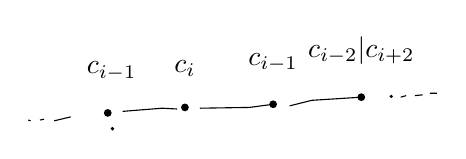
\begin{tikzpicture}[x=1cm,y=1cm]
\draw (-1.01,-.09)--(-.98,-.10) (-.86,-.09)--(-.81,-.08)
 (-.68,-.10)--(-.47,-.05);
\draw (.19,.02)--(.69,.06)--(.88,.05);
\draw (1.17,.06)--(1.80,.07)--(2.10,.11);
\draw (2.31,.09)--(2.59,.16)--(3.22,.20);
\fill (0,0) circle (1.4pt);
\fill (.98,.07) circle (1.4pt);
\fill (2.10,.11) circle (1.4pt);
\fill (3.22,.20) circle (1.4pt);
\fill (.06,-.20) circle (.7pt);
\fill (3.60,.21) circle (.65pt);
\draw (3.72,.20)--(3.79,.22) (3.90,.22)--(4.00,.23)
 (4.09,.25)--(4.18,.25);
\node[above] at (.05,.29) {$c_{i-1}$};
\node[above] at (.98,.34) {$c_i$};
\node[above] at (2.10,.40) {$c_{i-1}$};
\node[above] at (3.22,.49) {$\unsure{c_{i-2}|c_{i+2}}$};
\end{tikzpicture}}
et de
\figure{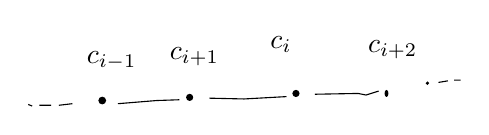
\begin{tikzpicture}[x=1cm,y=1cm]
\draw (-.94,-.05)--(-.89,-.07) (-.80,-.06)--(-.65,-.06)
 (-.55,-.06)--(-.38,-.04);
\draw (.20,-.04)--(.69,0)--(.98,.01);
\draw (1.36,.03)--(1.80,.02)--(2.34,.05);
\draw (2.70,.08)--(3.25,.09)--(3.35,.07)--(3.51,.12);
\fill (0,0) circle (1.4pt);
\fill (1.11,.04) circle (1.3pt);
\fill (2.46,.09) circle (1.3pt);
\fill (3.61,.09) ellipse (.025 and .045);
\fill (4.13,.22) circle (.65pt);
\draw (4.27,.23)--(4.39,.25) (4.47,.26)--(4.55,.26);
\node[above] at (.12,.26) {$c_{i-1}$};
\node[above] at (1.17,.32) {$c_{i+1}$};
\node[above] at (2.27,.48) {$c_i$};
\node[above] at (3.69,.40) {$c_{i+2}$};
\end{tikzpicture}}
en contractant la \deleted{\unsure{seg}} \inserted{arête} qui joint $c_i$ et $\unsure{c_{i-1}|c_{i+1}}$, OK.
\margin{74}

\scanpage{76}
\mspage{37}
9) \uline{La structure groupoïdale des} \inserted{\uline{espaces modulaires de}} \uline{Teichmuller} \uline{modules} (la MDT-structure) : cas transcendant, morphismes de générisation.

Nous travaillons maintenant avec les $M^{\mathrm{an}}_{g,\nu}$, $\widehat M^{\mathrm{an}}_{g,\nu}$ etc -- et pour ne pas traîner les exposants ``an'' (pour ``analytique''), nous les faisons tomber.

Considérons pour tout MD-graphe $\underline G$, la multiplicité modulaire (analytique) $M_{\underline G}$, et son groupoïde fondamental, que je note $\Pi M_{\underline G}$. C'est une \inserted{``grosse''} catégorie, par la suite nous allons voir comment \unsure{la|le} remplacer \inserted{\unsure{canoniq\textsuperscript{t}}} par une \deleted{catégorie} \inserted{groupoïde} dont l'ens des objets soit fini. Dans nos constructions, il est en effet licite de remplacer un groupoïde tel que $\Pi M_{\begin{tikzpicture}[baseline=(g.base),x=1ex,y=1ex]
\node[inner sep=0pt,outer sep=0pt] (g) at (0,0) {$\scriptstyle\underline G$};
\node[inner sep=0pt,outer sep=0pt,anchor=south] at (-0.08,0.25) {$\unsure{\begin{tikzpicture}[x=0.65ex,y=0.65ex,baseline=0pt]
\draw[line width=0.28pt] (0,0) -- (-0.11,1.18);
\draw[line width=0.28pt] (-0.04,0.59) -- (0.24,0.92);
\end{tikzpicture}}$};
\end{tikzpicture}}$ par un groupoïde équivalent, pourvu que \deleted{l'équivalence} \inserted{dans celui-ci} $\underset{\unsure{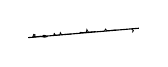
\begin{tikzpicture}[x=1em,y=1em,baseline=0pt]
\draw[line width=0.4pt] (0,0) -- (4.0,0.34);
\draw[line width=0.3pt] (0.16,0.015) -- (0.20,0.12) -- (0.25,0.10) -- (0.21,0.02)
 -- (0.35,0.04) .. controls (0.48,0.10) and (0.53,-0.04) .. (0.68,0.035)
 .. controls (0.59,0.12) and (0.51,0.08) .. (0.50,0.045);
\draw[line width=0.3pt] (0.92,0.08) -- (0.94,0.15) -- (0.99,0.08)
 -- (1.14,0.10) -- (1.16,0.18) -- (1.20,0.11) -- (1.56,0.13);
\draw[line width=0.3pt] (1.86,0.16) .. controls (1.88,0.26) and (1.90,0.14) .. (1.98,0.18)
 -- (2.10,0.20) -- (2.12,0.29) -- (2.17,0.20) -- (2.44,0.22);
\draw[line width=0.3pt] (2.76,0.24) -- (2.79,0.31) -- (2.85,0.25) -- (3.19,0.28);
\draw[line width=0.3pt] (3.73,0.32) -- (3.80,0.25) -- (3.76,0.19);
\end{tikzpicture}}}{\text{le groupe}}$
\[
(94)\qquad \Gamma_{\underline G}=\operatorname{Aut}\underline G
\]
opère, et que l'équivalence commute à l'\unsure{action} de ce groupe.

Notons déjà que $\Pi M_{\underline G}$ est un groupoïde
\margin{75}

\scanpage{77}
connexe, dont le $\pi_1$ est isomorphe en tant que \uline{groupe extérieur}) :
\diagram{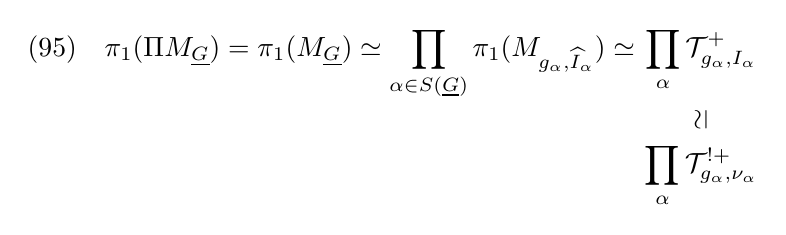
\begin{tikzpicture}[every node/.style={inner sep=0pt}]
\node[anchor=base east] (chain) at (0,0) {$\displaystyle(95)\quad\pi_1(\Pi M_{\underline G})=\pi_1(M_{\underline G})\simeq\prod_{\alpha\in S(\underline G)}\pi_1(M_{g_\alpha,\widehat I_\alpha})\simeq$};
\node[anchor=base west] (upper) at (0.12,0) {$\displaystyle\prod_\alpha\mathcal T^+_{g_\alpha,I_\alpha}$};
\node[rotate=90] at ([yshift=-0.35cm]upper.south) {$\simeq$};
\node[anchor=north] at ([yshift=-0.65cm]upper.south) {$\displaystyle\prod_\alpha\mathcal T^{!+}_{g_\alpha,\nu_\alpha}$};
\end{tikzpicture}}
\margin{où les $\mathcal T^{!+}_{g,\nu}$ sont des groupes de Teichmüller}
Les opérations de $\Gamma^{\unsure{!|\natural|\deleted{!}}}_{\underline G}$ sur $\Pi M_{\underline G}$ définissent un groupoïde mixte $(\Pi M_{\underline G},\Gamma_G)$, dont le groupe fondamental (extérieur) \unsure{s'insère} \deleted{\unsure{de} \unsure{par}} \inserted{dans une} structure d'extension
\[
(96)\quad1\longrightarrow\pi_1(\Pi M_{\underline G},\Gamma_{\underline G})\longrightarrow\pi_1(\Pi M_{\underline G},\Gamma_{\underline G})\relbar\joinrel\relbar\Gamma_G\longrightarrow1
\]
Nous allons définir une \inserted{sorte de} variance des $\Pi M_{\underline G}$ relativement à deux sortes de ``morphismes'' pour les MD-graphes $\underline G$. 

Tout d'abord une \uline{``variance de générisation''}, qui est composée de la \uline{variance pour isomorphismes} de MD-graphes (que j'admets comme ``triviale'', et qu'il est inutile de préciser) et une ``variance de passage au \unsure{quotient} de MD-graphes''.
\margin{76}

\scanpage{78}
\mspage{38}
Soit donc $\underline G'$ un MD-graphe quotient de $\underline G$ -- par un ens. \inserted{$C$} d'arêtes du graphe $G$ sous-jacent à $\underline G$,
\[
(96)\qquad\underline G'=\underline G/C.
\]
On a alors un \inserted{diagramme de} morphismes canoniques
\diagram{\begin{tikzpicture}[x=1cm,y=1cm]
\node at (-3.1,.85) {$(97)$};
\node at (0,1.8) {$\overset{\deleted{\unsure{\wedge}}}{M}_{\underline G}$};
\node at (3.0,1.9) {$\deleted{\unsure{\widehat M_{\underline G'}}}$};
\node at (0,0) {$\widehat M_{\underline G}$};
\node at (3.0,.12) {$\widehat M_{\underline G'}$};
\node at (1.48,1.80) {$\deleted{\longrightarrow}$};
\draw (.10,1.11) .. controls (.25,1.28) and (-.13,1.36) .. (-.13,1.10)
 -- (.02,.56);
\draw (3.12,1.24) .. controls (3.24,1.40) and (2.85,1.46) .. (2.87,1.20)
 -- (3.00,.65);
\draw (2.86,.82)--(3.00,.65)--(3.15,.84);
\draw (2.59,1.34)--(3.48,1.78)--(2.62,1.05)--(3.48,1.46)
 --(2.64,.73)--(3.46,1.12)--(2.70,.48);
\draw[->] (.86,.05)--(2.18,.10);
\end{tikzpicture}}
\margin{déployer la déf. de $\Gamma^!_{\underline G,\underline G'}$ !}
Si on désigne par $\Gamma^!_{\underline G,C}$ ou $\Gamma^!_{\underline G,\underline G'}$ le sous-groupe de $\Gamma_{\underline G}$ qui est formé des autom qui transforment $C$ en lui-$=$, et qui induisent l'identité sur $\underline G'$, \unsure{la flèche|l'hom.} \deleted{\unsure{verticale}} \inserted{horizontale} $\underset{\unsure{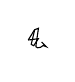
\begin{tikzpicture}[baseline=-.5ex,x=.10cm,y=.10cm]
\draw[line width=.4pt] (0,1)--(.8,2.3)--(1.3,2.5)--(1.0,.45)
 .. controls (.75,-.1) and (1.5,-.1) .. (1.9,.3)--(2.3,.15)--(1.7,.75);
\draw[line width=.4pt] (0,1)--(1.28,1.17)--(.70,.28)--(.38,.45)--(.82,2.30);
\end{tikzpicture}}}{\text{de}}$ (97) se factorise \deleted{\unsure{donc}} \inserted{une} immersion de multiplicités
\diagram{(98):\qquad\begin{tikzcd}[ampersand replacement=\&]
(\widehat M_{\underline G},\Gamma^!_{\underline G,\underline G'})\arrow[r,hook] \& \widehat M_{\underline G'}
\end{tikzcd}}
\margin{Ce ne sont peut-être que des immersions \uline{locales}, il me semble -- à vérifier\ldots}
Je désigne par $\widehat M_{\underline G,\underline G'}$ le \uline{germe de multiplicité} défini par l'inclusion (98), et par $M_{\underline G,\underline G'}$ le germe défini par l'inclusion induite
\diagram{(99)\qquad\begin{tikzcd}[ampersand replacement=\&]
(M_{\underline G},\Gamma^!_{G,G'})\arrow[r,hook] \& \widehat M_{\underline G'}
\end{tikzcd}}
\margin{Il vaut mieux considérer le germe de multiplicité défini par l'\uline{immersion locale} $M_{\underline G}\longrightarrow\unsure{M_{\underline G'}|\widehat M_{\underline G'}}$, et faire opérer $\Gamma^{\unsure{!}}_{\underline G,G'}$ dessus, \unsure{et ce sera} $M_{\underline G,\underline G'}$}
\margin{77}

\scanpage{79}
Je désigne par $\widehat M^*_{\underline G,\underline G'}$, $\overset{\unsure{\deleted{\wedge}}}{M}{}^*_{\underline G,\underline G'}$ les germes de multiplicités obtenus en \deleted{enlevant (``\unsure{l'infini|l'âme}'') $\widehat M_{\underline G}$ resp. $M_{\underline G}$, $\unsure{\Gamma^!_{\underline G,\underline G'}}$ (les traces \unsure{de la réunion|sur le germe} des diviseurs de $\unsure{\widehat M_{\underline G'}}$ \unsure{qui contiennent} $\unsure{(\widehat M_{\underline G},\Gamma^!_{G,G'})}$)}
\inserted{\deleted{\unsure{prenant les traces de} $M$} enlevant les traces des diviseurs à l'infini de $\widehat M_{\underline G'}$ \deleted{\unsure{non seuls}} qui contiennent $\widehat M_{\unsure{\underline G|G}}$ -- dans le cas de $M^*_{\underline G,\underline G'}$, on prend la \uline{trace} de $M_{\underline G'}$ sur $\widehat M_{\underline G,\underline G'}$}
\unsure{Ils sont donc} des filtres d'ouverts de la multiplicité $M_{G'}$, et les groupoïdes fondamentaux* \deleted{$\unsure{\Pi}$}
\[
(100)\qquad\Pi M^{\unsure{*|\leftarrow}}_{\underline G,\underline G'},\qquad\Pi M^{\unsure{*|\leftarrow}}_{\underline G,\underline G'}
\]
sont définis comme des Catégories $\underset{\longrightarrow}{\lim}$ des catégories de revêtements universels, \unsure{ou} ou comme des catégories des revêtts \unsure{du connexe} desdits germes de multi-plicités (comparer [5], n°5, p. $768'$).

On a alors des diagrammes de germes de multiplicités analytiques
\diagram{\begin{tikzpicture}[x=1cm,y=1cm]
\node[inner sep=2pt] (A) at (0,0) {$M^*_{\underline G,\underline G'}$};
\node[inner sep=2pt] (B) at (4,0) {$M_{\underline G'}\deleted{\unsure{M}}$};
\node[inner sep=2pt] (C) at (-2.6,-2) {$(M_{\underline G}\deleted{\unsure{,\Gamma^!}})$};
\node[inner sep=2pt] (D) at (0,-2) {$M_{\underline G,\underline G'}$};
\draw[line cap=round] ([xshift=4pt]A.east) -- ([xshift=-8pt]B.west);
\draw[->] ([yshift=-5pt]A.south) -- ([yshift=5pt]D.north);
\draw[->] (C.east) -- (D.west);
\node[anchor=east] at (-3.75,-1.05) {$(101)$};
\node[anchor=north west,inner sep=0pt] (caption) at (-1.65,-2.55) {(équiv d'homotopie !)};
\node[anchor=base west,inner sep=0pt] at ([xshift=5pt,yshift=5pt]caption.north east) {$\unsure{)}$};
\end{tikzpicture}}
donnant lieu \unsure{à|:} des morphismes de groupoïdes
\margin{78}
